\documentclass[11pt]{article}
\RequirePackage{mmap}%
\usepackage[a4paper, hmargin={2.8cm, 2.8cm}, vmargin={2.5cm, 2.5cm}]{geometry}
\usepackage{eso-pic} % \AddToShipoutPicture
\usepackage{graphicx} % \includegraphicsud over
\usepackage[utf8]{inputenc} % æøå
\usepackage[T1]{fontenc} % mere æøå
\usepackage{verbatim} % så man kan skrive ren tekst
\usepackage{listings} % kode
\usepackage[round]{natbib} %citationer i chicago format
\usepackage{amsmath} % flere matematikkommandoer
\usepackage[british,UKenglish,USenglish,english,american]{babel} % orddeling
\usepackage[all]{xy} % den sidste (avancerede) formel i dokumentet
\usepackage{graphicx} %for billedhåndtering
\usepackage{listings} %algoritmer og programming language
\usepackage{fancyhdr} %header, footer
\usepackage{hyperref}
\usepackage{multirow}
\usepackage{pdfpages}
\usepackage{multicol}
\usepackage{fancyhdr}
\usepackage{clrscode3e}
\usepackage{indentfirst}
\usepackage{wrapfig}
\usepackage{units}

\newcommand{\citat}[2]{\begin{justify}\textit{``#1''}\hspace{0.1cm}\footnote{#2}\end{justify}}
\author{
 \textsc{\Large{Valdas Zabulionis}}\\\\
 \textsc{\Large{Rune Franch Pedersen}}\\\\
 \textsc{\Large{Amr El Sayed}}\\}
\title{
  \vspace{3cm}
  \textsc{\Huge{Bachelor Project}}\\
  \vspace{0.5cm}
  \textsc{\Large{A Visualization Tool for Learning Algorithms and Datastructures}}\\
  \vspace{3cm}
  %\textsc{\Huge{\\Midtvejsrapport}}\\
 \textsc{\Large{2016 block 3-4}}
}
\begin{document}

%% Change `ku-farve` to `nat-farve` to use SCIENCE's old colors or
%% `natbio-farve` to use SCIENCE's new colors and logo.
\AddToShipoutPicture*{\put(0,0){\includegraphics*[viewport=0 0 700 600]{ku-farve}}}
\AddToShipoutPicture*{\put(0,602){\includegraphics*[viewport=0 600 700 1600]{ku-farve}}}

%% Change `ku-en` to `nat-en` to use the `Faculty of Science` header
\AddToShipoutPicture*{\put(0,0){\includegraphics*{kuen}}}

\clearpage\maketitle
\thispagestyle{empty}
\newpage
\begin{center}{\huge\textbf{A Visualization Tool for Learning Algorithms and Datastructures}}\newline \textit{\\DIKU - Bachelor Project}\end{center}
\hfill \break
\begin{tabular}{l l l }
\textbf{Studens Names} &: &Valdas Zabulionis - LHN100\\\\
&: &Rune Franch Pedersen - VQR730\\\\
&: &Amr El Sayed - VWJ159\\\\
\textbf{University} &:& University of Copenhagen\\\\
\textbf{Institution} &:& Department of Computer Science DIKU\\\\
\textbf{Supervisor} &:& Oleksandr Shturmov\\\\
\textbf{Period} &:& Block 3 - block 4\\\\
\textbf{Year} &:& 2016\\\\
\textbf{Pages} &:& \_\\
\end{tabular}
\\\\\\\\\\\\\\\\\\\\
\begin{center}{\huge\textbf{Certificate}}\end{center}

This is to certify that the work contained in the thesis entitled "A Visualization Tool for Learning Algorithms and Datastructures" by Valdas Zabulionis, Rune Franch Pedersen and Amr El Sayed, has been carried out under our supervision and that this work has not been submitted elsewhere.\\\\\\\\\\\\
\begin{center}\noindent\rule{8cm}{0.4pt}%\end{center}

\begin{center}
\textbf{Supervisor}\\
Oleksandr Shturmov \\
oleks@di.ku.dk \\
Department of Computer Science DIKU \\
University of Copenhagen
\end{center}
\newpage
\tableofcontents
\end{center}
\newpage

\section{Introduction}
%\addcontentsline{toc}{section}{Introduction}
\subsection{About the Project}
%\addcontentsline{toc}{subsection}{About the Project} 
A Visualization Tool for Learning Algorithms and Datastructures is a web-based learning tool conceptualized by Oleksandr Shturmov, Amr El Sayed, Valdas Zabulionis and Rune Franch Pedersen with the aims of improving teaching of data structures and algorithms through dynamic interactive visualizations. Students from Computer Science institute Copenhagen University may use our tool to help them with understand and implement algorithms. \\
The tool consists of two major components: the visualization component and the training component.

\subsection{Problem definition}
%\addcontentsline{toc}{subsection}{Problem definition}
For students, who are relatively unfamiliar with algorithms and programming, getting a comprehensive understanding of algorithms can be very difficult.\\
In this project we will design a visual tool to help student create their own basic algorithms and do a step-by-step run-through of them.
This is intended to help students learn the basics of algorithms.\\
The primary focus is an easy to use tool, which will use visual building blocks, that are predefined statements providing function body, statements, condition expressions, cases, loops, etc.. They can be easily used by the students to create an algorithm. The tool would also include a built-in function which will provide a detailed step-by-step description of each step in the implemented algorithm.
\subsection{Scope}
%\addcontentsline{toc}{subsection}{Scope}

%En koncis og præcis beskrivelse af det undersøgte problem.
%Denne kan efter aftale med vejleder afvige (lidt) fra
%beskrivelsen i synopsen.
%Scope/project limitations fra synopsen. Skal muligvis skrives lidt om?

We will only implement a few of the algorithms shown in the algorithm book(\citep{algbog}), with an emphasis on making it easy to support further extensions.

We will not estimate the running of the algorithms that the students implement, although it could be a part of the project. We have decided that we would leave the estimation of running time to the students to find on their own, since it is an important part of learning datastructures and algorithms.\\
It is not intended that the program executes arbitrary student code.\\
The primary documentation for our project will be our report.\\
We will only perform internal testing of the program, and will not include any outside users or resources for testing of the functionality.\\
The focus for our project will be to implement the program to work with the merge-sort algorithm. If the time allows, further functionality in the form of more algorithms will be implemented.

\section{Problem Analysis}
%\addcontentsline{toc}{section}{Problem Analysis}
%Problem analysis skal skrives rent ind/omformuleres

To create a program that helps students, we face many problems that have to be solved. The first and most important problem is to choose how the users gain access to the program, in other words how it is delivered.
\\

Second is the problem of implementation. We must choose the subjectively best tools for implementing the program. This problem contains the choices of programming languages.
\\

Another problem would be figuring out how the UI should look, so that it is relatively straightforward for the users to use, and at the same time it should be relatively straight forward to upgrade by adding new buttons, visuals or extending functionality.

Then there is the problem of making the UI frontend work with the backend.

\noindent How should the user interact with the program. How should they be able to create algorithms.\\
How to visualize an algorithm, how to show what is happening using graphics.\\
How to recognize what the user input is in the algorithm creation field, and how to compute it, and at the same time how to display it to the user (step-by-step).\\

\noindent This program is intended to be used by lecturers and teaching assistants as a tool for helping students to learn algorithms. It is important that the program could have a set of building blocks specific for each week of the course for the students to use. It is also very important that the the building blocks are easy to add, easy to be removed, and are easily edited to correct bugs. 
\section{Design}
%\addcontentsline{toc}{section}{Design}
%Skal skrives bedre 
To make it easier for students to have access to our \underline{program}, we have decided that it should be web-based --- meaning that the it should be accessed via internet by using a standard web browser. This way there would be no need to distribute the program and all of the required packages for it to run, as was our first thought. By making the \underline{program} web-based, we ensure the accessibility of it for most, if not all, users. The solution will not target mobile/tablet users specifically, but they should be able to use the website nonetheless.\\
The choice of programming language for our project is not a clear one. Because we decided to make it web-based, a possibility is to use JavaScript for the whole implementation, but we decided that the code itself would quickly become hard to decipher. So we thought of splitting the program into two parts --- the frontend and the backend. Frontend would be coded in HTML, CSS, and JavaScript, CSS/JavaScript framework like React, and the backend would be coded in a programming language of our choice.\\

For our project we had two programming languages in mind - Go \url{https://golang.org/} and Python. The reasoning for using Python is that we are relatively familiar with it, and we have used it before. Go on the other hand is a relatively new programming language and it is on it's way up in popularity, so it would have been interesting to learn it. Go features faster compile- and run-times than Python, and also supports a subjectively better framework for client-server interactions, all the while having high concurrency optimization.\\
Having these things in mind, we have chosen Python for our project, mainly because of two reasons. The first reason is that GO is not as dynamic as Python, and adding building blocks on-the-fly would be impossible without having to restart the server. The second reason is that we have limited time, and learning a new language could lead to delays in the production schedule.\\
%At the moment we have two programming languages in mind for our backend. One of them is Python. Python is a choice because we are relatively familiar with it, and it is easily coded. A downside would be, that we have heard that is it relatively complicated to write server-client packages and modify their contents.\\
%The other language that we have in mind is GO, which is quickly becoming a popular programming language. A pro for it is, that it is easier to handle server-client requests using GO. It would also be a good thing to learn one more programming language, especially one that is on the rise in popularity and may become one of the more used programming languages in the world.\\\\
\subsection{Designing the UI}
We have decided that the UI should be separated into three windows \ref{uiframes}. On the left, the user would have access to various blocks that could be dragged into the main window, which would be placed in the middle of the screen. These blocks would make up the various functionality that would make it possible for the user to create their algorithm. The main window would be like a notepad, where the user would try to implement their algorithm. On the right side, there would be a small window with a visualization component for showing what happens while running the algorithm step-by-step. Below it there would be a log window, where the user would see values of various variables and function calls.\\

%To solve the problem of communication between the frontend and the backend, we need to do some more background studies. We have a couple of ideas of how to implement function calls, what data packages and when to send them from the client to the server. We should have a clearer idea of how to solve this problem, when we have moved further along into the implementation process.\\

A big part of our project is to visualize what is happening when a given algorithm is being run. For example the students would like to build an implementation of the heap-sort algorithm. They would have the choice to select the heap-sort algorithm from a list of algorithm, and when they are finished implementing and would like to run the step-by-step program, they would be shown what happens in a heap at the same time that they are running their algorithm. This functionality would be done as most independent entity as possible, so that it would be possible to upgrade it at a later time, since we are only going to implement this only as a place-holder, so it won't look as good as it could if done with great care for the visual design.\\

How to recognize user input, and how to read their algorithm, this is still a work in progress. The idea is for users to click/drag-and-drop building blocks which would have fields where the users would write their input. This input would be saved client side for a fixed amount of time, and it would be sent as a series of instructions to the server. The order in which the building blocks would appear in the middle of the screen text field, would decide how the server would read and execute instructions it receives. The point of saving user input client side, is to ensure that their work progress is not lost if they suddenly lose internet connection. This would also help to decrease the connection load server side, so as not to have a constant stream of data, but only instructions being sent when requested or needed.

\subsection{Designing the Building Blocks}
An important aspect of this project is the requirement that is should be easy for an administrator of the program to add additional options for constructing a algorithm. That is, it should be possible add more functionality for a user to use in their algorithm, be it a new type of loop or an operator for strings or whatever the administrator wishes to add. Since the program It should also be possible to restrict the user access to certain functionality. 

\section{Inspiration}
To get some inspiration for our work, we tried to find similar projects to see how they have designed their layout and what kind of functionality they support.\\
Pythontutor  \citep{pythontutor} is a tool which lets the user execute Python code one step at a time, giving the users a visual representation (shown in figure \ref{pythontutor}) of what is happening while the code is running at a given step\citep{Guo:2013:OPT:2445196.2445368}.\\
\begin{figure}[h]
	\centering
	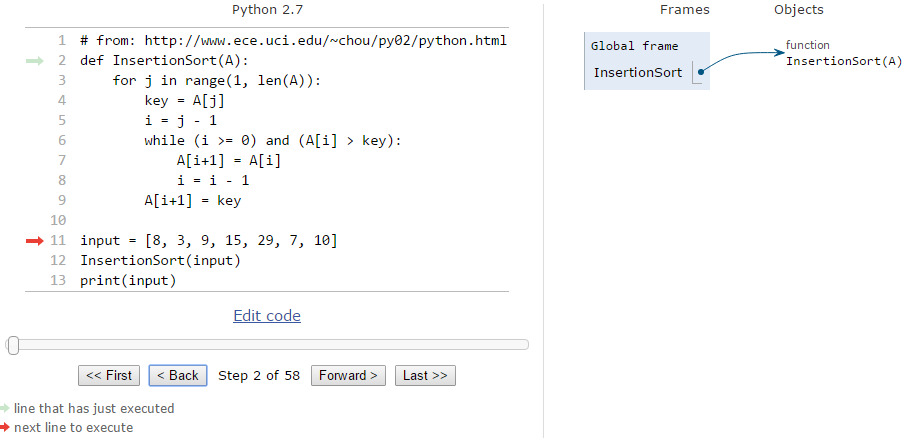
\includegraphics[scale=0.4]{img/pytutins1.PNG}
    \caption{Python tutor \url{http://pythontutor.com/}}
    \label{pythontutor}
\end{figure}\\
This is a fine example of a program that has a similar design to what we have imagined for our program, and we will strive to recreate some of its simplicity in our own program design.

\subsection{Blockly}
At a point in our implementation phase we stumbled upon a project called Blockly \citep{Blockly}. It is a library that may be embedded in an application and it adds an editor so that a user can use blocks that represent programming code to write their own programs, which then can be translated to a chosen programming language. Blockly is basically a programming language translator, that translates a code sequence created with their building blocks to any of the implemented languages.
\begin{figure}[h]
	\centering
	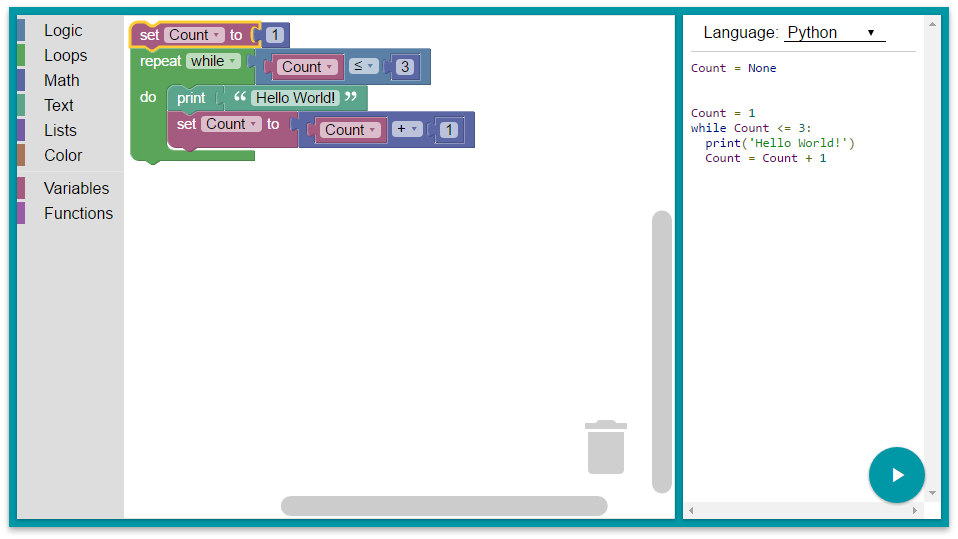
\includegraphics[scale=0.4]{img/blocklypy1.PNG}
    \caption{Blockly \url{https://developers.google.com/blockly/}}
    \label{Blockly}
\end{figure}\\
Blockly as seen in Figure \ref{Blockly} is quite similar to our project, as it is developed using Python and JavaScript, and it uses blocks to represent and visualize 
pseudo code.The biggest differences between Blockly and our project are that Blockly has been created with fancy visuals, and building blocks that can only be attached where they fit.\\
Another difference is that our project is designed to support new building blocks, and this can be done by adding them server side and reloading the webpage. To add new building blocks to Blockly, they would have to restart their entire server. It is also easier to implement new building blocks with our project, than it is with Blockly. We have chosen how a block should be written, and new blocks would only have to follow that template. New blocks in Blockly would not only have to be made from scratch, they also need graphics to be made for them before they can be used in the program.

\newpage
\section{Implementation}
%\addcontentsline{toc}{section}{Implementation}

\subsection{Building Blocks}
%\addcontentsline{toc}{subsection}{Building Block Grammar}
%Skal vi forklare tanken bag vores grammar?
% De skal også lige sættes op så de ikke ligner lort

The buildings blocks are implemented using python files. These files consist of a building block class, and the functionality to implement the algorithms and executing them is contained in this class. This includes the information on the design of the representation of object in the menu the building block is added from, as well as the representation of the block when it is added to the algorithm. A type for the building block and the code that is run, when the building block is executed, is also included in the building blocks.
These Python files are imported by the server using the BuildBlockManager function. The BuildBlockManager extracts the information from the files and processes it to functioning html code and JavaScript functions. 
The Building Block class is made up of these four following functions and should be made in the same style if more are to be added.\\
\textbf{show\_in\_menu:}\\
This function contains the HTML code for how the building block should look in the menu. This code is wrapped in a <div> box by the BuildBlockManager function and added to the menu containing the blocks. This <div> box is made draggable and is given the python file's name as an id, and the id is therefore automatically unique, before being added to the menu.\\
The building blocks, we have implemented, is made up of multiple <div> boxes in the same design as they will be represented when added to the algorithm. An empty box, which is used to add other building blocks into, all use the same style as seen in the picture ??????. %add picture of contain style
\textbf{show\_in\_screen:}\\
The HTML code, which is how the building block is reprensented when added to the algorithm, is extracted from this function. The BuildBlockManager uses this code to generate the insert function, as described in section ?????. This code is appended to <div> box the building block is dropped on.\\
When the HTML contains a box into which it should be possible to drop another building block, it must call the drop or dropLines functions, described in section?????, as these are the functions that append other building blocks to the boxes.
\textbf{funtionality??:}\\
\textbf{type??:}\\
%The building blocks are intended to be files written in Python. Each file will contain the code needed for the creation of it's own button on the interface. The interface will automatically include all the files that match a predefined blueprint, that we provide, thereby making it possible to easily add further functionality to our system. These files will be server-side and only people with SSH access to the server should be capable of adding more functionality. The button added by the file will allow a user of our system to add a function or value to the algorithm that the user is trying to implement, this could be a loop, binary operator or whatever the one who has written the file wishes too implement, as long as it fits the blueprint. We will add the needed building blocks to implement a few basic algorithms. The grammar discussed below are how we intend to implement the building blocks we design. \\\\
%The building blocks will need to include all the information that is needed by the interface to process the functionality of the button. Therefore it is necessary for the building blocks to contain the information for the button, the mathematics that the functionality needs to perform and the text for the algorithm as well as the log.
%The class diagram in figure \ref{bbclassdia} is for the building blocks and though it is an early version, it should give an idea of the layout for the building blocks.\\
%As shown a building block must contain two attributes and three operations that can be executed. The attributes in question are a name and a type. By dividing the building blocks up in certain types we can ensure that we avoid situations where we get nonsense code in the algorithm, like a while loop that doesn't contain a Boolean value for it's condition statement. We also intend to give the building blocks a hierarchy, that will force the user to do things in a certain order thereby making it easier implement the backend. The name is the name that will appear on the button and should be of the string type. A maximum size for the this attribute might also be a good idea to implement. The type is used to make it possible to describe a specific grammar used by the building blocks, this is done by type checking on each building block. This type attribute should be of the string type. The first two operations, show\_in\_menu and show\_in\_screen, where screen is middle section -- the pseudo-code/algorithm container, are used by the interface to generate the HTML code for the button, and the text that is added to the algorithm container screen when the button is activated. The last operation is used to add the button's functionality to a document that will be used by the step-by-step function to visualize the algorithm. \\\\
%We have completed the definition of the building block grammar of the building blocks we will implement. There might be some improvements or corrections at a later date, but this should as close to the final version as possible. 
\newpage
\begin{codebox}
\zi \proc{Procedure} $::= \id{ProcName} \;\;'(\;'\; \id{Args} \;'\;)'$
\zi \quad\quad\quad\quad\quad\quad\quad Lines
\zi \proc{Args} $::= \id{ValName} ',' Args$
\zi \quad\quad\quad| \id{ValName}
\zi \proc{Lines} $::= \id{Line}\; '\backslash n'\; \id{Lines}$
\zi \quad\quad\quad| Line
\zi \proc{Line} $::=$'\id{return}' \id{Expr}
\zi  \quad\quad\quad| \proc{Procname} '(' Args ')'
\zi \quad\quad\quad| \id{Expr}
\zi \proc{Expr} $::=\left \lfloor{\id{Expr}}\right \rfloor  $
\zi \quad\quad\quad| $\left \lceil{\id{Expr}}\right \rceil $
\zi \quad\quad\quad| \id{Expr} 'Binary Operator' \id{Expr}
\zi \quad\quad\quad| \id{Value}
\zi \quad\quad\quad| \id{ValName}
%\zi \quad\quad\quad| \id{Value} \id{ValName}
\zi \quad\quad\quad| $'['\id{Values}']'$
\zi \proc{Array} $::=[\id{Values}]$
\zi \proc{Values} $::= \id{Values} ',' Value$
\zi \quad\quad\quad| \id{Value}
\zi \proc{Value} $::= \id{Const}$
%\zi \quad\quad\quad| \id{Const}
%\zi \quad\quad\quad| \id{Const} \id{ValName}
\zi \proc{Loop} $::= $'\id{for}' (\id{Statement})
\zi \quad\quad\quad\quad Lines
\zi \quad\quad\quad| '\id{while}' '(' \id{Statement} ')'
\zi \quad\quad\quad\quad Lines
\zi \proc{Statement} $::=$ \id{Expr} 'Boolean Operator' \id{Expr}
\zi \quad\quad\quad| \id{Statement} 'AND' \id{Statement}
\zi \quad\quad\quad| \id{Statement} 'OR' \id{Statement}
\end{codebox}

\newpage
\subsection{UI}
For the implementation of the user interface we have chosen to use Bootstrap. Bootstrap is a front-end framework for web development. This tool helps us flesh out the user interface, ensuring that it looks the same no matter what browser the user is using to access the website.\\
\begin{wrapfigure}{r}{0.6\textwidth} %this figure will be at the right
    \centering
    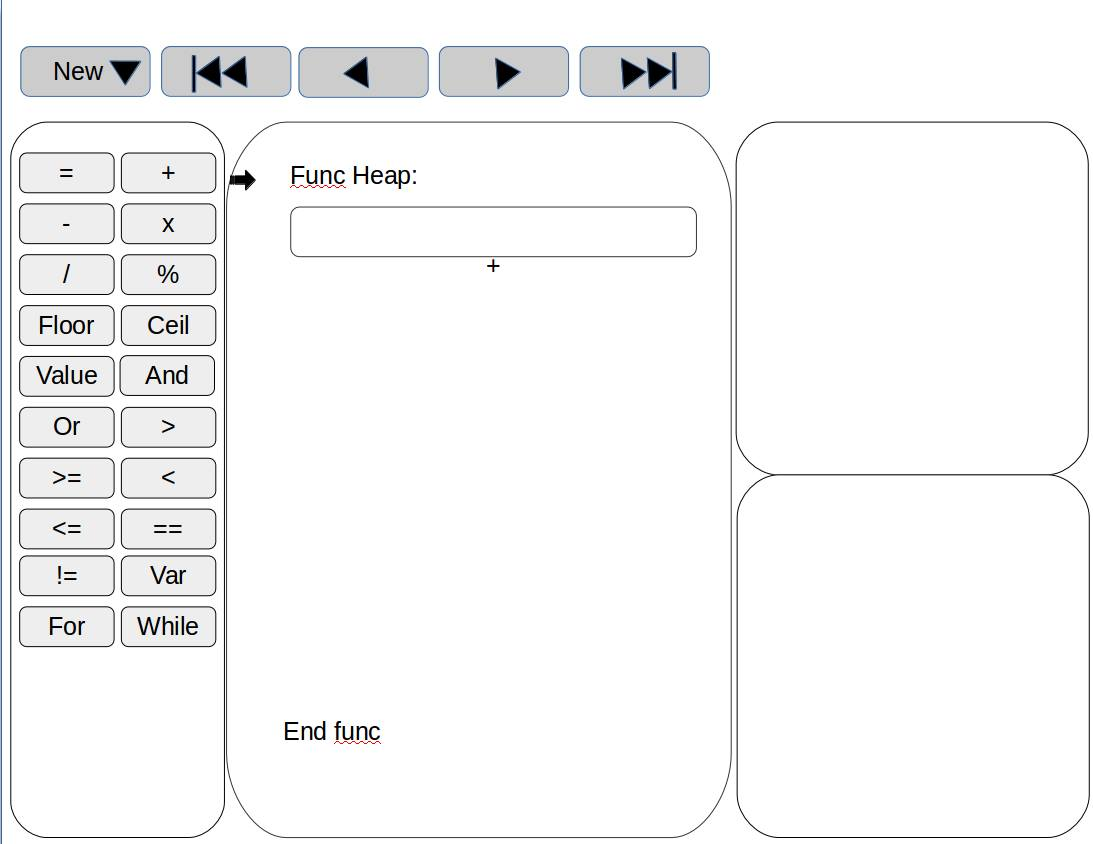
\includegraphics[width=0.5\textwidth]{img/ui_1.png}
    \caption{UI wireframes}
    \label{uiframes}
\end{wrapfigure}
\\
The interface will support further extension of the implemented buttons and will be able to support new buttons used to create the algorithms. The interface is intended to use some functionality to include files from the server, which represent the buttons, that are the building blocks discussed below. We are still designing this functionality to enable the communication between the client and the server, which will automatically generate the building blocks to client interface. How a building block is displayed in the client, depends on the definitions that are contained in each block.\\\\
Figure \ref{uiframes} 'UI wireframes' shows the main idea of how our UI will look. The top navigation bar holds the control buttons, which provide the interaction part of this application to allow clients to start new algorithm and control the step-by-step run of their code.
The left section is where the building block buttons are placed. These buttons will be automatically generated to the UI from the first GET request. The middle section is the pseudo-code container and here the users will write their algorithms by using the building block buttons. The pseudo-code container will highlight the current code, using a colored box, and if the clients need to start new instruction, then they have to click the add new line button located at the bottom of the highlight box. This will highlight the newly created line below the previous instruction. The top window on the right will be used for a table containing all the variables currently in the algorithm. And the bottom window on the right a log for the step-by-step function.

\subsection{Server}

\subsection{The webpage}

\subsubsection{UI??}

\subsubsection{Left menu}
Left menu is where we have visual representations of our building blocks in the form of draggable HTML <div> objects. Users may choose which building block they need to build their pseudo code, and insert the said object in to the pseudo code container by dragging and dropping them on the container.\\
The left menu is populated with items when the webpage is accessed, and those items are created server-side from all of the available building blocks for the given assignment week. Item generation is handled by the building block manager, which was mentioned in the server section. The way that the left menu items look are defined in the building blocks themselves, so their visualization is not strictly controlled, and gives way for easy customization if changes to the way they look are requested.\\
Left menu has a fixed size of \nicefrac{1}{3} 

\subsubsection{JavaScript}

\subsubsection{Pseudo code container}

\subsubsection{Log Container}

\subsection{Step-by-step}

\subsection{Import and export}

\newpage
\section{Work progress}
%\addcontentsline{toc}{section}{Work Progress}
%Status for det hidtidige arbejde og tidsplan for resten af forløbet.
At this point in time we have partially completed the first work task which was to design and implement the interface for our program. We have mostly completed the graphical design of the program, and what is left is to connect the HTML code to our backend, all the while adding some finishing touches to the visual representation of the interface.\\
We have completed the grammar needed to create building blocks, and this should probably be the final version of the grammar that we will be using in our program.\\
This is the link to our Github.\\
https://github.com/Amr116/AlgTool
\\
\subsection{Time schedule}
%\addcontentsline{toc}{subsection}{Time Schedule}
We have fallen a bit behind schedule with implementing the interface, and this could mean delays for the rest of our schedule. The implementation of building blocks could be moved a week back. The same goes for the import/export functionality, since this should be done after implementing the building blocks. Other than that, our work schedule is pretty much not unchanged.

\begin{itemize}
\item{Building blocks - date changed to 27/4 from 20/4}
\item{Import/export - date changed to 01/5 from 23/4}
\item{Step-by-Step simulation - date unchanged 15/5}
\item{Pretty print - date unchanged 01/6}
\end{itemize}

The current delay could mean that the implementation of our step-by-step simulation being delayed as well, but we still should have time buffer after our last item (the pretty-print) before our deadline to mitigate any further delays.
\newpage

\iffalse

\subsection{Time schedule and work tasks}
%\addcontentsline{toc}{subsection}{Time schedule and work tasks}
\noindent\makebox[\linewidth]{\rule{\paperwidth}{0.4pt}}
\begin{center}\textbf{Work assignments}\end{center}
\noindent\makebox[\linewidth]{\rule{\paperwidth}{0.4pt}}

\noindent\textbf{Definition}: Interface\\
\textbf{Product}: graphics and backend for the application interface.\\
\textbf{Resource Requirement}: open source language ( python, java script, HTML, CSS ) to implement the product, and browser to visualize the product. \\
\textbf{Dependencies}: This work task can be completed without any of the other work tasks having been implemented.\\
\textbf{Time Required}: 2-3 work days.\\
\textbf{Deadline}: 1 / 04/ 2016\\
\noindent\makebox[\linewidth]{\rule{\paperwidth}{0.4pt}}

\noindent\textbf{Definition}:  Grammar \\
\textbf{product} : definition of the building blocks syntax\\
\textbf{Resource Requirement}: Introduction to Compiler Design - Torben Ægidius Mogensen \citep*{mogensen2011introduction}\\
\textbf{Dependencies}: This work task can be completed independently of the other tasks.\\
\textbf{Time Required}: 1-2 work days\\
\textbf{Deadline}: 1/ 04/ 2016\\
\noindent\makebox[\linewidth]{\rule{\paperwidth}{0.4pt}}

\noindent\textbf{Definition}: Building Blocks \\
\textbf{Product}: graphics and backend for the buttons used for creating the algorithms as well as implementing them in the interface.\\
\textbf{Resource Requirement}: open source language ( Python, JavaScript, HTML, CSS ) to implement the product, and browser to visualize the product. \\
\textbf{Dependencies}: This work task needs the finished implementation of the interface and the parser to be completed.\\
\textbf{Time Required}: 5-6 work days\\
\textbf{Deadline}: 20/ 04/ 2016\\
\noindent\makebox[\linewidth]{\rule{\paperwidth}{0.4pt}}

\noindent\textbf{Definition}: Import and Export \\
\textbf{Product}: The ability to save code written in the program and export it as a file, so that it may be distributed and imported on a different machine.\\
\textbf{Resource Requirement}: open source language ( Python, JavaScript, HTML, CSS ) to implement the product, and browser to visualize the product. \\
\textbf{Dependencies}: This work task needs the finished implementation of the interface and the building blocks.\\
\textbf{Time Required}: 1-3 work days\\
\textbf{Deadline}: 23/ 04/ 2016\\
\noindent\makebox[\linewidth]{\rule{\paperwidth}{0.4pt}}

\noindent\textbf{Definition}:  Step-by-Step Simulation\\
\textbf{product}: graphics and backend for the step by step  algorithms simulation, as well as implementing them in the interface.\\
\textbf{Resource Requirement}: open source language ( Python, JavaScript, HTML, CSS ) to implement the product, and browser to visualize the product. \\
\textbf{Dependencies}: This work task depends on the complete implementation of the interface.\\
\textbf{Time Required}: 5-6 work days\\
\textbf{Deadline}: 15/ 05/ 2016\\
\noindent\makebox[\linewidth]{\rule{\paperwidth}{0.4pt}}

\noindent\makebox[\linewidth]{\rule{\paperwidth}{0.4pt}}
\noindent\textbf{Definition}:  Pretty Print\\
\textbf{product}: graphics and backend for printing the variables results and the return results of the functions, as well as implementing them in the interface.\\
\textbf{resource requirement}: open source language ( Python, JavaScript, HTML, CSS ) to implement the product, and browser to visualize the product. \\
\textbf{Dependencies}: This work task needs the finished implementation of the interface to be completed.\\
\textbf{Time Required}: 8-10 work days\\
\textbf{Deadline}: 01/ 06/ 2016\\
\noindent\makebox[\linewidth]{\rule{\paperwidth}{0.4pt}}

\fi

\addcontentsline{toc}{section}{References}
\bibliographystyle{unsrtnat}
\bibliography{ref}
%\nocite{Guo:2013:OPT:2445196.2445368}
\nocite{foutsitzis2010teaching}
\url{https://scratch.mit.edu/}\\
\nocite{Blockly}
\\\\\\\\\\\\\\\\\\
%\begin{tabular}{ l l l c r l l l}
%~\ ~\ \textbf{Student Signature} & & & & & & ~\ ~\ ~\ ~\ ~\ ~\ ~\ ~\ ~\ ~\ ~\ \textbf{Supervisor Signature}\\\\
%~\ ~\ ~\ Valdas Zabulionis & & & & & & ~\ ~\ ~\ ~\ ~\ ~\ ~\ ~\ ~\ ~\ ~\ ~\ Oleksandr Shturmov\\\\\\\\
%~\ ~\ ~\ Rune Franch Pedersen & & & & & & \\\\\\\\
%~\ ~\ ~\ Amr El Sayed & & & & & &
%\end{tabular}
\end{document}
